%%%%%%%%%%%%%%%%%%%%%%%%%%%%%%%%%%%%%%%%%%%%%%%%%%%%%%%%%%%%%%%%%%
%%    Vorlage für wissenschaftliche Arbeiten an der TU Berlin   %%
%%    -------------------------------------------------------   %%
%%                 Erstellt von Felix Reich, M.Sc.              %%
%%                    UTF-Version, Stand (2013)                 %%
%%                                                              %%
%%  Bedienung der Vorlage anhand der Dateien:                   %%
%%   - Projekteinstellungen  (Titel, Name, Datum, ...)          %%
%%   - Kommandos  (Eigene und vorgefertigte Makros)             %%
%%   - Silbentrennung  (Für Wörter, die falsch getrennt sind)   %%
%%   - Glossar  (= Wörterbuch)                                  %%
%%   - Symbole  (Formelzeichen für Verzeichnis)                 %%
%%   - Abkuerzungen (Für Abkürzungsverzeichnis)                 %%
%%   - FrontMatter  (Inhaltsverzeichnis, Titelseite, ...)       %%
%%   - BodyMatter  (WICHTIG! Hier mit \include aus dem Ordner   %%
%%                  Inhalt seine Kapitel einfügen)              %%
%%   - BackMatter  (Abbildungsverzeichnis, etc.)                %%
%%       WICHTIG: Front- und Backmatter unbedingt individuell   %%
%%       anpassen über Ein- Auskommentieren von Anweisungen     %%
%%   - Anhang  (insofern vorhanden, hier mit \include einfügen) %%
%%                                                              %%
%%  Es sind drei verschiedene KOMA-Klassen verwendbar:          %%
%%  - scrartcl -scrreprt (standard) -scrbook                    %%
%%  Zum Ändern in der Datei Klasse die documentclass und den    %%
%%  logischen Schalter anpassen.                                %%
%%                                                              %%
%%  Es wird empfohlen, die anderen Dateien möglichst wenig      %%
%%  zu modifizieren. Neulinge im wissenschaftlichen Satz        %%
%%  sollten die Dokumente im Verzeichnis Hilfe studieren, um    %%
%%  ein ästhetisch ansprechendes Ergebnis zu erzielen.          %%
%%                                                              %%
%% Wer eps-Dateien einbinden möchte, muss bei pdflatex          %%
%%    --shell-escape für tetex oder texlive bzw.                %%
%%    --enable-write18 für miktex übergeben.                    %%
%%                                                              %%
%% Zur Verwendung der Verzeichnisse Index, Glossar, Abkürzungen %%
%% und Symbole muss respektiv makeindex aufgerufen werden mit:  %%
%% -s "Index/Index.ist -i Dokument.idx -o Dokument.ind          %%
%% -s Dokument.ist -t Dokument.glg -o Dokument.gls Dokument.glo %%
%% -s Dokument.ist -t Dokument.alg -o Dokument.acr Dokument.acn %%
%% -s Dokument.ist -t Dokument.slg -o Dokument.sym Dokument.sbl %%
%%%%%%%%%%%%%%%%%%%%%%%%%%%%%%%%%%%%%%%%%%%%%%%%%%%%%%%%%%%%%%%%%%
%% ADAPTED BY MAXIMILIAN WEBER, 2017-2019                       %%
%%%%%%%%%%%%%%%%%%%%%%%%%%%%%%%%%%%%%%%%%%%%%%%%%%%%%%%%%%%%%%%%%%

% Dokumentklasse mit Basiseinstellungen
% Dokumenteneinstellungen werden hier vorgenommen. Tiefere Layout-Einstellungen folgen separat.

% Hier u. a. auch möglich: 
% Spaltenanzahl (onecolumn, twocolumn)
% Kapitel nur auf rechten Seiten beginnen oder auf jeder (openright, openany)
% Beginn von Absätzen (parindent, halfparskip, parskip)

\documentclass[
headings=big,  						% Überschriftengröße (möglich: small, normal und big)
captions=tableheading,				% Tabellen-Captions als Überschriften formatieren
bibliography=totoc,			% Fügt das Literaturverzeichnis im Inhaltsverzeichnis hinzu
listof=totoc,						% Fügt die weiteren Verzeichnisse im Inhaltsverzeichnis hinzu
index=totoc,						% Fügt auch den Index im Inhaltsverzeichnis hinzu				
draft=false,							% Graphiken werden gesetzt. bei draft=true sind Graphiken nur als Rahmendummies verfügbar
numbers=noenddot				% keine Punkte nach kapitelnummern un so
]{scrreprt} 					  	% Wählen aus scrartcl, scrreprt und scrbook !!! Unten unbedingt den Schalter anpassen !!!
% Logische Schalter für Dokumentenklasse 
\def\typeScrartcl{1}  % Für scrartcl
\def\typeScrreprt{2}  % Für scrreprt
\def\typeScrbook{3}   % Für scrbook

% !! Schalter hier setzen, damit die Vorlage korrekt funktioniert !!
\let\doctype=\typeScrreprt

% Projektdefinitionen
\usepackage[utf8]{inputenc}
%\usepackage[russian,german,ngerman]{babel}

% Titelei
\newcommand*{\Titel}{Efficient Singing Voice Synthesis}
\newcommand*{\PdfTitel}{Efficient Singing Voice Synthesis}
\newcommand*{\Untertitel}{Master Thesis Proposal}
% Header-Titel
\newcommand*{\HeaderTitel}{Master Thesis Proposal}

% Hauptautor
\newcommand*{\Autor}{William Rodewald}
\newcommand*{\AutorMatrikelNr}{372193}

% Manuell gesetztes Datum mit Ort
\newcommand*{\Datum}{Berlin, \today}

% Uni, Fakultät, Institut und Fachgebiet
\newcommand*{\Uni}{Technische Universität Berlin}
\newcommand*{\Fakultaet}{Fakultät I}
\newcommand*{\Institut}{Institut für Sprache und Kommunikation}
\newcommand*{\Fachgebiet}{Fachgebiet Audiokommunikation}

% Professor und Betreuer
\newcommand*{\Professor}{Prof. Dr. Stefan Weinzierl}
\newcommand*{\BetreuerA}{Dr. Henrik Hahn}
\newcommand*{\InstitutA}{Fachgebiet Audiokommunikation}
\newcommand*{\InstitutB}{Ableton AG}

% Weitere Autoren 
%\newcommand*{\AutorB}{William Rodewald}
%\newcommand*{\AutorBMatrikelNr}{372193}

%\newcommand*{\AutorC}{Maximilian Weber}
%\newcommand*{\AutorCMatrikelNr}{385153}


% Gruppenangabe oder nur "vorgelegt von:" schreiben.
\newcommand*{\Gruppe}{vorgelegt von:}

% Einstellen der Druckversion: Drucken oder PDF-Ansicht allein
\def\typeDrucken{1}  % Für Drucken (nicht ändern)
\def\typePDFonly{2}  % Für reine PDF-Verwendung (nicht ändern)
% Hier den passenden Schalter setzen! =\typeDrucken oder =\typePDFonly
\let\pdftype=\typePDFonly

% Definition, ob ein- oder zweiseitig gesetzt werden soll
\def\typeOnepage{1}  % Für einseigen Satz
\def\typeTwopage{2}  % Für zweiseitgen Satz
% Hier den passenden Schalter setzen! =\typeOnepage oder =\typeTwopage
\let\pagetype=\typeOnepage

% Bindekorrektur am inneren Rand
\newlength{\bindCorrection} 				%Deklaration, nicht ändern
\setlength{\bindCorrection}{0cm} 			%Zuweisung, kann geändert werden

% PDF-Ausgabe-Version über Minor-Nummer => 1.x
\pdfminorversion=5
\pdfcompresslevel=9

% Paket-Definitionen und deren Einstellungen
% Einstellung der Eingabe (Zeichensatz, Sprache, ...)
% Sichert die Copy&Paste-Fähigkeit
\usepackage{cmap}

% Korrekte Darstellung europäischer Zeichen wie Umlaute
\usepackage[OT2, T1]{fontenc}
% Beispiel: Ohne dieses Paket wäre ein ä eine Kombination von: a + . + . = drei Zeichen -> schlecht für Copy & Paste aus der PDF und für die Suche

% Einstellung des Eingabezeichensatz
\usepackage[utf8]{inputenc}
% Gewählt: UTF-8-Zeichensatz (für Windows: ansi nehmen)

% Umlaute bei Overleaf! (Max W)
%\usepackage[utf8x]{inputenc}
%\usepackage[german]

% Translation verschiedener Elemente des Dokumentes
%\usepackage[german,ngerman]{babel}
%\usepackage[ngerman]{babel}
%\addto{\captionsngerman}{%
%	\renewcommand{\bibname}{Quellenverzeichnis}
%}

% ENGLISH (M. Weber)
\usepackage[english]{babel}

% Z. B. die korrekte Übersetzung von Verzeichnisnamen. Mehrere Namen als Option sind möglich. Die zuletzt geladene Sprache ist standard, sollte ngerman (Deutsch mit Reformanpassung) sein.


% Ermöglicht Silbentrennung von zusammengesetzten Wörtern
\usepackage[shortcuts]{extdash}
% Z. B.: \hyphenation{Berta} \hyphenation{Ra-ke-te} Berta\-/Rakete
% Siehe Datei Silbentrennung

% Textsatz-Einstellungen
% Anpassen der Tiefe von nummerierten Überschriften. In wissenschaftlichen Dokumenten ist es üblich, bis zur dritten Ebene zu nummerieren. Da die Klassen verschiedene Hauptebenen (\chapter oder \section) haben, muss individuell angepasst werden!
\ifcase\doctype 
  \or \setcounter{secnumdepth}{3} % Für scrartcl
  \or \setcounter{secnumdepth}{2} % Für scrartcl
  \or \setcounter{secnumdepth}{2} % Für scrbook
\fi

% Vermeidung von Umbruchproblemen nach Axel Reichert
\tolerance 1414
\hbadness 1414
\emergencystretch 1.5em
\hfuzz 0.3pt
\widowpenalty=10000
\vfuzz \hfuzz
\raggedbottom 

% Falls bei Arbeiten Absätze durch Zeilenabstand und uneingerückte neue Zeilen erforderlich sind:
\setlength{\parindent}{0pt}	 % kein Einzug bei neuem Absatz
\setlength{\parskip}{0.5ex plus0.5ex minus 0.5ex} % Abstand zwischen 2 Absätzen 
%\setlength{\parskip}{0.2pt}
% Zeilenabstand einstellen
\usepackage{setspace}
%\singlespacing % Ist i. d. R. auch standardmäßig aktiv
\onehalfspacing
% Alternativ für einige Arbeiten gefordert: \onehalfspacing oder \doublespacing

% Verschiedene Hilfspakete
% Paket für schnellen Beispieltext zum Füllen
%\usepackage{blindtext}
% Aus der Hilfe:
% \blindtext creates some text,
% \Blindtext creates more text.
% \blinddocument creates a small document with sections, lists...
% \Blinddocument creates a large document with sections, lists...

% Gant Diagram  (MAX)
\usepackage{pgfgantt}

% Linebreak in Table
\usepackage{makecell}

% Tabellen
\usepackage{tabularx,ragged2e}
%\newcolumntype{C}{>{\Centering\arraybackslash}X}

% Wichtige Macro-Definitionen 
\usepackage{etoolbox}
% Z. B. wichtig für logische Abfragen:
% \ifstrequal{String}{Vergleichstring}{...passiert when gleich}{...ansonsten}
% Anderes Beispiel, s. "Anpassen der Tiefe von nummerierten Überschriften" in Satzeinstellungen

% Weitertes Macro-Paket. Zwar depreciated, dennoch benötigt, da es in Skripten Kommandos auflöst
\usepackage{ifthen}
% Bsp: \ifthenelse{\equal{\kommando1}{\kommando2}}{true}{false}

% Ermöglicht das Verwenden von Listen mit kleineren vertikalen Abständen
\usepackage{mdwlist}
% Statt itemize einfach itemize* verwenden. Analog dazu existiert enumerate* und description*
% Diese Umbegungen erlauben auch Unterbrechungen, z. B.  mit \suspend{itemize*} bla bla \resume{itemize*}

%Bei Itemize davor und danach größere Abstände
\usepackage{enumitem}
\setlist[itemize]{topsep=5pt}

%Das gleiche für Quotes
\usepackage{quoting}
\quotingsetup{vskip=5pt}

% Ermöglicht erweiterte Referenzen. Soweit angepasst, dass schöne Makros möglich sind (siehe Kommando-Definitionen)
\usepackage[english]{varioref}
\renewcommand*{\reftextfaraway}[1]{auf S.\,\pageref{#1}}%
\renewcommand*{\reftextcurrent}{\unskip}%
% generell neu: \vpageref, \vref und \vref*, diese Referenzierungen geben die Seite mit an

% Ermöglichung von Unterabbildungen
\usepackage{subfig}
% Verwendung in figure: \subfloat[Optionaler Verzeichnistext][Unterschrift \label{sfig:bla}]{...Zeug...}

% Das normgerechte Eurozeichen
\usepackage{eurosym}
% Verwendung mit \euro

% Kommandos nach Ende einer Seite absetzen
\usepackage{afterpage} 
% Wichtigste Anwendung ist das Flushen von Floats: \afterpage{\clearpage}

 % Nassi-Schneidermann Unterstützung
%\usepackage{Template/Pakete/nassi}
%\setiftext{W}{F}
%\nassiwidth=\textwidth
% Wichtige Befehle:
% \NSD{}
% \WHILE{Text}{} \ENDWHILE
% \ACTION{Text}

% Einrahmen von Text
%\usepackage{framed}
%\addtolength{\FrameRule}{1pt} % dickeren Rahmen
% Verwendung: \begin{framed} ... \end{framed}

%Anhang
\usepackage[title]{appendix}

%Runden
\usepackage{xparse}

\ExplSyntaxOn
\DeclareExpandableDocumentCommand \ceil { O{0} m }
{ \fp_eval:n { ceil(#2,#1) } }
\ExplSyntaxOff

\ExplSyntaxOn
\DeclareExpandableDocumentCommand \floor { O{0} m }
{ \fp_eval:n { floor(#2,#1) } }
\ExplSyntaxOff

% Table Caption Distance
\usepackage{caption}
\captionsetup[table]{skip=10pt}

% Max Weber
\usepackage[nodayofweek]{datetime}
\usepackage{layouts}
\usepackage{mathrsfs}


\usepackage{floatrow}

% nicer inverse
\newcommand{\inv}{^{\raisebox{.2ex}{$\scriptscriptstyle-1$}}}

% Layout-Einstellungen
% Hier sind Layoutoptionen zu finden, die aus Übersichtsgründen nicht in der Datei "Klasse.tex" eingefügt sind

% Serifenschrift 
% Ersetzt Computer Modern mit Latin Modern, sieht aber nahezu gleich aus. Grund ist die mangelnde Unterstützung von korrekt gesetzten Umlauten und die Lesbarkeit am Monitor.
\usepackage{lmodern}

% Fügt Symbole zum Font hinzu, die in Latin Modern nicht enthalten sind, wie z. B. das Euro-Symbol
\usepackage{textcomp}

% Ersetzt die Schreibmaschinen-Schrift und verwendet Adobe Courier statt Latin Modern oder Computer Modern
\usepackage{courier}

%Farbe
%\usepackage[x11names]{xcolor}

% Optischer Randausgleich
\usepackage{microtype}
% Wenn man die Augen zukneift, kann man ohne diesem Paket bei Blocksatz auf der rechten Seite "Dellen" erkennen, da Punkte und Striche vor der virtuellen Trennlinie gehalten werden. Dieses Paket ermöglicht kleine Übertretungen, die das optische Bild verbessern.

% Setzt die Schriftgröße. Ebenfalls soll die Titelseite separat gesetzt werden
\KOMAoptions{
fontsize=11pt,			% Schriftgröße. Standard = 11pt
titlepage=true			% Separat gesetzte Titelseite verwenden
}
%Serifenschrift für Überschriften
\setkomafont{sectioning}{\normalfont\normalcolor\bfseries}

% Verwendung des geometry Packets für die Einstellung des Papierformats / Seitenabstände / Bindekorrektur
\usepackage[
a4paper, 													% DIN A4-Papier
\ifcase\pagetype \or twoside=false \or twoside=true \fi , 	% Ein- oder zweiseitig 
bindingoffset=\bindCorrection,								% Binde-Korrektur
bottom=3.35cm													% unterer Rand
]{geometry}
\setlength{\footskip}{1cm} %Fußzeile tiefer

%Jede Section neue seite (blöd bei chapterbeginn)
%\let\oldsection\section
%\renewcommand\section{\clearpage\oldsection}

% Header und Footer für ein- oder zweiseitigen Satz über das Paket scrpage2 einstellen
\usepackage[automark, headsepline, footsepline, plainfootsepline, plainheadsepline, ilines]{scrpage2}
\setlength{\headheight}{1.1\baselineskip} % Max W. ?
\pagestyle{scrplain}
\clearscrheadfoot
\ifcase\pagetype
\or % Für einseitigen Satz

% HEADER / FOOTER
\lohead[\Untertitel]{\Untertitel}
\rohead[\pagemark]{\pagemark}
\lofoot[{\scriptsize \leftmark}]{
\ifthenelse{\equal{\leftmark}{\rightmark}}
	{\scriptsize \rightmark}
{
	\ifthenelse{\equal{\rightmark}{}}
		{\scriptsize {\leftmark}}
		{\scriptsize {\leftmark} -- {\rightmark}}
}
}
\or % Für zweiseitigen Satz
% Odd
\rohead[\pagemark]{\pagemark}       % right odd head
\lohead[\leftmark]{\leftmark}   % left odd head
% Even
\rehead[\PdfTitel]{\Untertitel}     % right even head
\lehead[\pagemark]{\pagemark}       % left even head

%\lehead[\rightmark]{\rightmark}     % left even head
%\refoot[{\scriptsize {\leftmark}}]{{\scriptsize {\leftmark}}}
%\lofoot[{\scriptsize {\rightmark}}]{{\scriptsize {\rightmark}}}
\fi

% Je nach gewählter Klasse das left- und rightmark anpassen
\ifcase\doctype 
\or % Für scrartcl
\addtokomafont{section}{\thispagestyle{scrplain}}
\renewcommand{\sectionmark}[1]{\markright{}\markleft{Abschnitt\ \thesection\ #1}{}}
\renewcommand{\subsectionmark}[1]{\markright{#1}{}}
\or % Für scrreprt 
%\addtokomafont{pagehead}{\scshape} %Kapitälchen in Header und Footer
\renewcommand{\chaptermark}[1]{\markright{}\markleft{\chaptername\ \thechapter\ #1}{}}
\renewcommand{\sectionmark}[1]{\markright{#1}{}}
\or % Für scrbook
\renewcommand{\chaptermark}[1]{\markright{}\markleft{\chaptername\ \thechapter\ #1}{}}
\renewcommand{\sectionmark}[1]{\markright{Abschnitt\ \thesection.\ #1}{}}
\fi

%Mathe in Überschriften fett
\makeatletter
\g@addto@macro\bfseries{\boldmath}
\makeatother

% Römische Ziffern im ToC sind sonst falsch aligned
\usepackage[tocindentauto]{tocstyle}
\usetocstyle{KOMAlike}
\settocstylefeature{pagenumberbox}{\hbox}

\usepackage[format=hang,justification=raggedright]{caption}


% Verschiedene Einstellungen zur Darstellung von Graphiken
% Einbinden von Vektor- und Rastergraphiken
%\usepackage[pdftex]{graphicx}
%\usepackage[space]{grffile}

%\graphicspath{{"D:/fabian sicherung/Uni-Master/Masterarbeit/Dokument/Bilder/pdf/"}{"D:/fabian sicherung/Uni-Master/Masterarbeit/Dokument/Bilder/jpg/"}}
%Hier Pfad ändern für kleinere Bilder
%\graphicspath{{"D:/fabian sicherung/Uni-Master/Masterarbeit/Dokument/Bilder/pdf/"}{"D:/fabian sicherung/Uni-Master/Masterarbeit/Dokument/Bilder/jpg/komprimiert/"}}


% Beispiel einer Anwendung: 
%\begin{figure}[!htb] % <<<---- Am besten hier positionieren, sonst oben oder unten auf der Seite
%\centering   % <<<---- Zentrierte Darstellung
%\includegraphics[width=1.00\textwidth]{beispiel.pdf}  % <<<---- Fügt auf ganze Seitenbreite das Bild "beispiel.pdf" ein
%\caption{Beispielbild}  % <<<---- Bildunterschrift
%\label{fig:marke}  % <<<---- Marke zum Referenzieren
%\end{figure}

% Ermöglicht die Verwendung von eps-Graphiken
%\usepackage{epstopdf}
% Dieses Paket wandelt on-the-fly eps-Dateien in pdf-Dateien um, diese werden in dem Bilder-Ordner automatisch abgelegt!
% Benötigt \write18 enabled, d. h. --shell-escape für tetex, texlive oder --enable-write18 für miktex

%Einbinden von Tikz und pgf, so dass auch sehr große 3D-Grafiken dargestellt werden können
\usepackage{tikz,pgfplots}
\usetikzlibrary{spy} %Vergrößerung
%PGFPLot-Optionen in Reihenfolge: Kompatibilität, deutsche Zahlentrennzeichen, runde Graphecken, dickere Graphen (0.4 is standard), kleinere Zahlen an Achsen, Hintergrund leicht blau, Rahmen etwas dicker, Grid, NaNs nicht zeichnen, x-Achse nicht enlargen
\pgfplotsset{compat=1.5, /pgf/number format/use comma,  every axis plot post/.append style={line join=round}, every axis plot/.append style={line width=1 pt}, axis background/.style={fill=blue!3}, axis line style = thick, grid=major, unbounded coords=jump, enlarge x limits=false}%every axis plot post/.append style={mark=none}},/pgf/number format/fixed,

%Legendensachen: Strichstärke, vert. Abstand Zeilen, Schrift links ausrichten, minor ticks kürzer
\pgfplotsset{
legend image post style={line width=1pt},
legend style={row sep=2pt},
legend cell align=left,
minor tick length=0.1cm* 0.8,
minor x tick num=1,
minor y tick num=1
}

%Schriftgrößen
\pgfplotsset{
	tick label style={font=\footnotesize},
	label style={font=\small},
	legend style={font=\small}
}

%Color Cycle List für PGF
\pgfplotscreateplotcyclelist{mycolorlist}{%
	blue\\%
	red\\%
	green!60!black\\%
	cyan\\%
	orange\\%
	magenta\\%
	violet\\%
	lime\\%
	black\\%
}

\usetikzlibrary{pgfplots.external,pgfplots.colormaps,decorations.markings,chains,fit,shapes,decorations.pathreplacing,positioning}
\usepgfplotslibrary{patchplots,colormaps}

%Makro für colormap reversen
\makeatletter
\def\customrevertcolormap#1{%
	\pgfplotsarraycopy{pgfpl@cm@#1}\to{custom@COPY}%
	\c@pgf@counta=0
	\c@pgf@countb=\pgfplotsarraysizeof{custom@COPY}\relax
	\c@pgf@countd=\c@pgf@countb
	\advance\c@pgf@countd by-1 %
	\pgfutil@loop
	\ifnum\c@pgf@counta<\c@pgf@countb
	\pgfplotsarrayselect{\c@pgf@counta}\of{custom@COPY}\to\pgfplots@loc@TMPa
	\pgfplotsarrayletentry\c@pgf@countd\of{pgfpl@cm@#1}=\pgfplots@loc@TMPa
	\advance\c@pgf@counta by1 %
	\advance\c@pgf@countd by-1 %
	\pgfutil@repeat
	%\pgfplots@colormap@showdebuginfofor{#1}%
}%

\makeatother

%pfdpages für Titelblatt muss vor externalize und dort auch "ausgeschlossen" werden durch optimize
\usepackage{pdfpages}

%Funktionierende, Scheiss-Methode:
%\tikzexternalize[shell escape=-enable-write18, prefix=Bilder/externalized/, optimize command away=\includepdf]

%Intervall zeichnen
\usepackage{tikz-dimline}

%alle neu machen...
%\tikzset{external/force remake}

% Mathematik-Pakete
% Wichtige Befehle zum schönen Mathesatz
\usepackage{amsmath}
% Umgebungsbeispiele: \equation, \align, \multline, \split, \boxed
% Kontrollkommandos: \subequations, \displaybreak, \intertext, \left, \right, \text
% Matrizen: matrix, pmatrix (), bmatrix [], Bmatrix {}, vmatrix ||, Vmatrix ||||
% u. v. m.

% Schriftarten zum Mathesatz
\usepackage{amsfonts}
% Z. B. \mathbb{R} für die reellen Zahlen

% Riesige Liste von mathematischen Symbolen und Operatoren
\usepackage{amssymb}
% Z. B. \in, \leq, \geq, \not, \sim, \approx, ...

% Weitere Symbole
\usepackage{stmaryrd}
% Z. B. \llbracket .. \rrbracket

% Unterdrückt unlogische Warnungen von stmaryrd
\SetSymbolFont{stmry}{bold}{U}{stmry}{m}{n}

% Für Theoreme
\usepackage{amsthm}
%\newtheorem{lemma}{Lemma} 
%\begin{lemma}
%...
%\end{lemma}

% Eine weitere Liste mit Symbolen, die häßlichere ablösen
\usepackage{latexsym}
% Z. B. \leadsto

% Normgerechtes Setzen von Zahlen mit SI-Einheiten
\usepackage[locale=DE]{siunitx}

%\usepackage[%per=slash,
%decimalsymbol=comma,
%loctolang={DE:ngerman,UK:english},
%]{siunitx}

\sisetup{exponent-product=\cdot,load-configurations=binary}
% \unit[1]{kg} = \SI{1}{\kilo\gram} == \SI{1}{kg} -> $1\,\text{kg}$
% \num{2.3d-2} -> $2,3 \cdot 10^{-2}$
% Stellt ebenfalls neuen Spaltentyp für Zahlen in Tabellen bereit für Ausrichtung am Dezimalzeichen:
% S[key=value, key=value, ...]
% Möglich sind hier z. B.:
% table-format = +3.2e+4 für 2 Vorkomma-, 4 Nachkomma- und 3 Exponentialstellen
% table-number-alignment=center oder right (Wo soll das Komamzeichen ausgerichtet werden?)
% table-figures-exponent=true oder false (Sollen die Exponenten auch ausgerichtet werden?)
% Weiterer neuer Spaltentyp s[key=value, ...] für Einheiten
% Wichtig hier: Kopfzeilen mit Text in {Text} versehen, bei mehreren Wörtern mit \multicolumn{1}{c}{Text} arbeiten. 

% Ermöglicht das Durchstreichen von Termen
\usepackage{cancel}
% \cancel{4}

% Verschiedene Möglichkeiten, Text zu unterstreichen. Wird in dieser Mathe-Datei eingefügt, da dieses Paket primär für Matrizen und Vektoren genutzt wird
\usepackage[normalem]{ulem}
% Z. B. für Vektoren \uline{v} oder für Matrizen \uuline{m}
% Aber auch für Text: \uwave{wellig}, \sout{falsch}, \xout{entfernt}, \dashuline{- - - }, \dotuline{. . . }

% Repariert die kaputte Kommasetzung für deutsche Kommazahlen im Mathemodus. Ursprünglich setzt Tex nach jedem Komma ein kleines Leerzeichen, aus 3,7 wird daher 3,\,7 = falsch.
\usepackage{icomma}
% Jetzt geht das Schreiben von 3,7 ohne Tricks. Ab jetzt nach Kommata mit -- gewünschten -- Abständen in Formeln ein Leerzeichen setzen, LaTex setzt dann ein kleines \,

% Setzen von Einheiten
\usepackage{units}
% Ermöglicht \unit[Zahl]{Einheit} und \unitfrac[Zahl]{Zähler}{Nenner} sowie nur \nicefrac{a}{b}
% Nicefrac setzen im Text statt a/b mit einem einfachen Slash die Terme abgesetzt.

% Darstellung von gerade gesetzten griechischen Buchstaben
\usepackage{upgreek}
% Verwendung z. B. mit: \uppi für ein gerades \pi

% Tensor-Notation / Indizes mit Abständen
\usepackage{tensor}
% Verwendung: M \indices{^a_b^{cd}_e}

% Erweiterter Blackboard-font
\usepackage{bbm}
% Verwendung: \mathbbm{N} - geht auch mit \boldsymbol

% Neue und überarbeitete Integralzeichen, ebenfalls bessere Abstände bei Mehrfachintegralen
\usepackage{esint}
% Verwendung: Z. B.: \oint

% Wurzel abschließen
\usepackage{letltxmacro}
\makeatletter
\let\oldr@@t\r@@t
\def\r@@t#1#2{%
\setbox0=\hbox{$\oldr@@t#1{#2\,}$}\dimen0=\ht0
\advance\dimen0-0.2\ht0
\setbox2=\hbox{\vrule height\ht0 depth -\dimen0}%
{\box0\lower0.4pt\box2}}
\LetLtxMacro{\oldsqrt}{\sqrt}
\renewcommand*{\sqrt}[2][\ ]{\oldsqrt[#1]{#2}}
\makeatother

% Gleichungsnummerierung
\ifcase\doctype 
\or \numberwithin{equation}{section}
\or 
\or  
\fi 

%Gleichstrom
\newcommand{\mathdirectcurrent}{\mathrel{\mathpalette\mathdirectcurrentinner\relax}}
\newcommand{\mathdirectcurrentinner}[2]{%
	\settowidth{\dimen0}{$#1=$}%
	\vbox to .85ex {\offinterlineskip
		\hbox to \dimen0{\hss\leaders\hrule\hskip.85\dimen0\hss}
		\vskip.35ex
		\hbox to \dimen0{\hss
			\leaders\hrule\hskip.17\dimen0
			\hskip.17\dimen0
			\leaders\hrule\hskip.17\dimen0
			\hskip.17\dimen0
			\leaders\hrule\hskip.17\dimen0
			\hss}
		\vfill
	}%
}
\newcommand{\textdirectcurrent}{\mathdirectcurrentinner{\textstyle}{}} 

% Tabellenpakete
% Tabellen mit fester Gesamtbreite
\usepackage{tabularx}
% Beispiel: \begin{tabularx}{6cm}{lrX} <- X ist die variable Größe

% Mehrseitige, lange Tabellen
\usepackage{longtable}
% Wichtig: Setzen von \endfirsthead, \endhead, \endfoot, \endlastfoot am Anfang nach \begin{longtable}

% Ermöglichung von gedrehten Tabellen
\usepackage{rotating}
% gedrehte Tabelle mit der neuen Float-Tabellenumgebung \begin{sidewaystable} erstellen

% Professionelles Tabellenlayout
\usepackage{booktabs}
% Ermöglicht die Verwendung von \toprule, \midrule, \bottomrule, \cmidrule
% Wichtig für wissenschaftlich und ästhetisch ansprechende Tabellen


%Columntype, den ich haben will
\newcolumntype{M}[1]{>{\centering\arraybackslash}m{#1}}

\usepackage{array}
\newcolumntype{L}[1]{>{\raggedright\let\newline\\\arraybackslash\hspace{0pt}}m{#1}}
\newcolumntype{C}[1]{>{\centering\let\newline\\\arraybackslash\hspace{0pt}}m{#1}}
\newcolumntype{R}[1]{>{\raggedleft\let\newline\\\arraybackslash\hspace{0pt}}m{#1}}


\usepackage[skip=0.5\baselineskip]{caption}


%Damit die scheiss Tabellen nicht mehr rumspringen
\usepackage{float}

% Float-Anpassungen
% Neudefinition der Tabellen- und Abbildungsunterschriften
\addto\captionsngerman{
% Abb. statt Abbildung in Bildunterschriften
\renewcommand{\figurename}{Fig.}
% Tab. statt Tabelle
\renewcommand{\tablename}{Tab.}
}
% Ändern des Abstandes zwischen den Abkürzungen Abb. bzw. Tab. und der jeweiligen Nummer von ~ auf \,
\renewcommand*{\figureformat}{\figurename\,\thefigure\autodot}
\renewcommand*{\tableformat}{\tablename\,\thetable\autodot}

% Kein Einzug ab der zweiten Caption-Zeile
\setcapindent{0em}

% Abkürzungen Abb. und  Tab. mit Nummer in den Floats fett setzen
\setkomafont{captionlabel}{\bfseries}

% Bild- und Tabellenunterschriften verkleinern
\addtokomafont{caption}{\small}

% Vorschlag für besseres Float-Placement von http://mintaka.sdsu.edu/GF/bibliog/latex/floats.html
\renewcommand{\topfraction}{0.9}				% Max. Anteil von Floats oben
\renewcommand{\bottomfraction}{0.8}				% Max. Anteil von Floats unten
\setcounter{topnumber}{2}						% Zwei Floats oben möglich
\setcounter{bottomnumber}{2}					% Zwei Floats unten möglich
\setcounter{totalnumber}{4}     				% Max. Anzahl Flaots auf einer Seite
\setcounter{dbltopnumber}{2}    				% Wie topnumber für zwei Spalten
\renewcommand{\dbltopfraction}{0.9}				% Wie topfraction für zwei Spalten
\renewcommand{\textfraction}{0.07}				% Min. text mit Floats
\renewcommand{\floatpagefraction}{0.7}			% Floatanteil, ab dem es Extraseiten gibt
\renewcommand{\dblfloatpagefraction}{0.7}		% Analog zu floatpagefraction für zwei Spalten


% Listings
% Änderungen, um Listings in KOMA korekt darzustellen (repariert die Floats)
\usepackage{scrhack}

% Listings-Unterstützung
\usepackage{listings}

% Bennenung der Caption und des Verzeichnisses
\renewcommand*\lstlistingname{Lst.\!}
\renewcommand*\lstlistlistingname{Template/Listings}

\lstset{
breaklines=true,		% Automatischer Umbruch
basicstyle=\scriptsize		% Etwas kleinerer Text als in der Umgebung
}

% Ein Beispiel:
%\begin{lstlisting}[float, language=C, label=lst:01, caption={Ein C-Beispiel}, frame=trBL]
%int main()
%{
%	int i;
%	for (i = 1; i < 10; i++)
%		printf("%i",i);
%	return(0);
%}
%\end{lstlisting}

% Bibliographie
% Wissenschaftliches Zitieren
%\bibliographystyle{unsrtnat} 
%\usepackage[sort&compress,numbers]{natbib}
\usepackage[numbers]{natbib}

%Absatz im Quellenverzeichnis
%\usepackage{natbibspacing}
%\setlength{\bibspacing}{10pt}


% Anpassen des Zitierstils
\bibpunct{[}{]}{,}{n}{}{,~}
% Eckige Klammern verwenden, mehrere Quellenangbaben durch Simikolon trennen, Autor-Jahr-Zitierweise verwenden (a), Zwischen Autor und Jahr kein Zeichen einfügen sowie bei Unterdrückung der mitarbeitenden Autoren ein Komma verwenden

% Naturwissenschftlicher der DIN angelehnter Zitierstil
%\bibliographystyle{natdin}	
%\bibliographystyle{abbrvdin}
\bibliographystyle{Content/Bibliographie/IEEEbib}

% PDF- und Linkeigenschaften
% Ermöglicht die Erweiterung von pdf-Dateien mit Links und Ähnlichem.
\usepackage{hyperref}
% Wenn Linkstellen im Text farbig sein sollen oder gar Formeln gesetzt werden, \texorpdfstring nutzen
% Mit \hypersetup werden die Schalter dieses Pakets weiter modifiziert

% Dokumenttitel setzen
\hypersetup{pdftitle={\PdfTitel}}

% Autor setzen
\hypersetup{pdfauthor={\Autor}}

% Thema setzen
\hypersetup{pdfsubject={\Untertitel}}

% Einstellung der Linkfarben (Drucken oder reine PDF-Ansicht)
\ifcase\pdftype 
\or % Für Drucken
\hypersetup{ %Alles was hier drin ist, muss für die hässlichen Boxen einkommentiert werden
    colorlinks=true,
    citecolor=black,
    filecolor=black,
    linkcolor=black,
    menucolor=black,
    urlcolor=black
}
\or % Für reine PDF-Verwendung
\hypersetup{
    colorlinks=true,
    linkcolor=black,
    anchorcolor=black,
    citecolor=black,
    filecolor=black,
    menucolor=black,
    urlcolor=black
}
\fi

% Einstellung, was das Inhaltsverzeichnis als Link verwenden soll
\ifcase\pdftype 
\or % Für Drucken
\hypersetup{linktoc=all}
\or % Für reine PDF-Verwendung
\hypersetup{linktoc=page}
\fi

% Einstellen der Bookmarks
\hypersetup{
bookmarksopen=true,
bookmarksnumbered=true
}

% Setzt Links korrekt für Floats (Fixt, das Labels nicht mehr am Ende stehen müssen)
\usepackage[all]{hypcap}

% Schönere URL-Formatierung (Für BibTeX und Text) von http://www.kronto.org/thesis/tips/url-formatting.html
\makeatletter
\def\url@leostyle{\@ifundefined{selectfont}{\def\UrlFont{\sf}}{\def\UrlFont{\small\ttfamily}}}
\makeatother
\urlstyle{leo}
% Manuelles Hinzufügen einer URL mit \url{www.narf.com}

% ??
% \usepackage[author={Maximilian Weber}]{pdfcomment}


% Glossar-Einstellungen
% Glossar laden - mit Abkürzungsverzeichnis 
\usepackage[acronym, toc]{glossaries}
% Später aufrufen: makeindex -s Dokument.ist -t Dokument.glg -o Dokument.gls Dokument.glo

% Symbolverzeichnis einstellen
\newglossary{symbols}{sym}{sbl}{Symbolverzeichnis}

% Üebrsetzen von Glossar und Abkürzungsverzeichnis
%\deftranslation[to=ngerman]{Acronyms}{Abkürzungsverzeichnis}
%\deftranslation[to=ngerman]{Glossary}{Glossar}

% Entfernen von Punkten hinter den Verzeichniseinträgen
\renewcommand*{\glspostdescription}{}

% Glossar festsetzen
\makeglossaries
% Als standard kein Kommentar bei Symbolen (später überschreibbar)
\newcommand{\symbComm}{}

% Style für Symbolverzeichnis
\newglossarystyle{symb3spaltig}{
% Umgebung: longtable 
\renewenvironment{theglossary}
{\symbComm{} \begin{longtable}{@{}p{1.5cm}p{1.5cm}p{\dimexpr\linewidth-1.5cm-1.5cm-4\tabcolsep\relax}@{}}} 
{\end{longtable}}
% Tabellenkopf 
\renewcommand*{\glossaryheader}{ 
\toprule 
\textbf{Symbol} & \textbf{Einheit} & \textbf{Beschreibung} \\ %Beschriftung 
\midrule 
\endhead}% 
% keine Überschriften zwischen Gruppen 
\renewcommand*{\glsgroupheading}[1]{}
% Haupteinträge in einer Zeile: 
\renewcommand*{\glossaryentryfield}[3]{
\glsentryuseri{##1}% Symbol 
& \glsentryuserii{##1}% Einheit 
& ##3% Beschreibung 
\\% Zeilenende 
}
% nichts zwischen Gruppen 
\renewcommand*{\glsgroupskip}{}% 
} 

% Ausgabe:
% Glossar: 			\printglossary[style=index]
% Abkürzungen: 	\printglossary[type=\acronymtype,style=list]
% Symbole:			\printglossary[type=symbols,style=list]

% Beispiele für die Verwendung

% Für einen Glossareintrag:
% \newglossaryentry{wagen}{name=Wa-gen,description={Macht Brum Brum},plural=Wa-gen,sort=wagen} 
% Dereferenzierung: \gls{wagen} (klein) \Gls{wagen} (fängt groß an) \GLS{wagen} (Kapitalschrift) \glspl{wagen} (Plural) ...\Glspl. \GLSpl - Referenz ohne Text: \glsadd
% Anderes Bsp.: \newglossaryentry{ohm}{name=ohm,symbol={\ensuremath{\Omega}},description=unit of electrical resistance}

% Für eine Abkürzung: 
% \newacronym{led}{LED}{light-emitting diode}

% Für Symbolverzeichniseintrag:
% \newglossaryentry{pi}{type=symbols,name={\ensuremath{\pi}},sort=pi, description={ratio of circumference of circle to its diameter}}

% Index-Einstellungen
% Index Erstellung
\usepackage{makeidx}

% Verweise auf andere Index-Einträge als deutsche Abkürzung
\renewcommand{\seename}{s.}

% Index festsetzen
\makeindex

% Achtung: makeindex muss folgendermaßen aufgerufen werden:
% makeindex -s "Index/Index.ist -i Dokument.idx -o Dokument.ind
%  Argument z. B. bei TexNicCenter im Postprozessor als
% -s "Index/Index.ist -i "%bm.idx" -o "%bm.ind"

% Beispiele für die Anwendung
% \index{hello} 							hello, 1 						Einfacher Eintrag
% \index{hello!Peter} 	  		Peter, 3 						Untereintrag von 'hello'
% \index{Sam@\textsl{Sam}} 		Sam, 2 							Formatierter Eintrag (Sortierung vorm @)
% \index{Lin@\textbf{Lin}} 		Lin, 7 							Wie zuvor
% \index{Jenny|textbf} 				Jenny, 3 						Formateirte Seitenzahl
% \index{Joe|textit} 					Joe, 5 							Wie oben
% \index{ecole@\'ecole} 			école, 4 						Sonderzeichen behandeln
% \index{Peter|see{hello}} 		Peter, s. hello 		Kreuzreferenz



%Abkürzungsverzeichnis
%\usepackage[printonlyused]{acronym}
\usepackage{acronym}
%\Auch für Formelzeichen benutzt, dann nur ohne printonlyused

\newcommand{\acrounit}[1]{
	\acroextra{\makebox[18mm][l]{{#1}}}
}

%Abkürzungen in der Auflistung fett -> auskommentieren 
\renewcommand*{\aclabelfont}[1]{\normalfont{\normalsize{#1}}\hfill}


%Ausländische Abkrüzungen
\makeatletter
\newcommand{\acroforeign}[1]{}

% patch the environment to print the foreign definition:
\AtBeginEnvironment{acronym}{%
	\def\acroforeign#1{ (#1)}%
}

% patch the acronym definition to safe the foreign definition:
\patchcmd\AC@@acro
{\begingroup}
{\begingroup\def\acroforeign##1{\csdef{ac@#1@foreign}{##1, }}}
{}
{}

% renew the first output to include the foreign definition if given:
\renewcommand*{\@acf}[1]{%
	\ifAC@footnote
	\acsfont{\csname ac@#1@foreign\endcsname\AC@acs{#1}}%
	\footnote{\AC@placelabel{#1}\hskip\z@\AC@acl{#1}{}}%
	\else
	\acffont{%
		\AC@placelabel{#1}\hskip\z@\AC@acl{#1}%
		\nolinebreak[3] %
		\acfsfont{(\acsfont{\csname ac@#1@foreign\endcsname\AC@acs{#1}})}%
	}%
	\fi
	\ifAC@starred\else\AC@logged{#1}\fi
}
\makeatother


% Eigene Kommandos
% Hier benutzerdefinierte Kommandos einfügen. Einige vordefinierte Kommandos sind unten zu finden.

\newcommand{\e}[1]{\mathrm{e} #1}
\renewcommand{\i}[1]{\mathrm{i} #1}
% Erstellt den diag-Operator 
\DeclareMathOperator{\diag}{diag}
% Erstellt eine partielle Ableitung (oben und unten ein \partial)
\newcommand{\pfrac}[2]{\frac{\partial #1}{\partial #2}}
%Zweite partielle Ableitung
\newcommand{\pfractwo}[2]{\frac{\partial^2 #1}{\partial {#2}^2}}
% "Totale" Ableitung
\newcommand{\tdfrac}[2]{\frac{\mathrm{d} #1}{\mathrm{d} #2}}
% Differentiale am Integralende
\renewcommand{\d}{\,\mathrm{d}}
% "Partial"-Zeichen
\newcommand{\p}{\partial}
% Fette Symbole (auch griechische)
%\newcommand{\bs}[1]{\boldsymbol{#1}}
% Betrag
\newcommand{\abs}[1]{\left\lvert #1 \right\rvert}
% Norm
\newcommand{\norm}[1]{\left\lVert #1 \right\rVert}
% Divergenz
\DeclareMathOperator{\divv}{div}
% Gradient
\DeclareMathOperator{\grad}{grad}
% Rotation
\DeclareMathOperator{\rot}{rot}
% Cofaktor
\DeclareMathOperator{\cof}{Cof}
% Spur
\DeclareMathOperator{\Spur}{Sp}
% Sprungklammer
\newcommand{\jump}[1]{\left \llbracket #1 \right \rrbracket}
%Signum-Funktion
\newcommand{\sign}{\text{sign}}
% Physikalische Komponenten
\newcommand{\phy}[1]{{\langle #1 \rangle}}
% Inverse eines Symbols, mit angepasster virtueller Höhe,
% damit Indizes passen (z. B. \inverse{\sigma}^{ij} )
\newcommand{\inverse}[1]{\stackrel{-1}{#1}\!\!\vphantom{#1}}
% Repariert kaputte Einrückungen, z. B. nach aligns
\newcommand{\fixIndent}{ \\[-\parskip]}
% Abkürzungen zum Erstellen von Gleichungen
\newcommand{\beq}{\begin{equation}}
\newcommand{\eeq}{\end{equation}}
\newcommand{\beqq}{\begin{equation*}}
\newcommand{\eeqq}{\end{equation*}}
\newcommand{\bal}{\begin{align}}
\newcommand{\eal}{\end{align}}
% Formelzeichen mit untergesetzter Formel (oder Zeichen), mit Indexhöhenanpassung.
\newcommand{\sU}[2]{\underset{#2}{#1}\vphantom{#1}}
% Wie oben, ignoriert aber beim Satz die Breite der Formel
\newcommand{\sUs}[2]{\smash{\underset{#2}{#1}\vphantom{#1}}}

% Neue Referenzbefehle über varioref (kein fancyref, da dies keine Abkürzungen vorsieht)
\newcommand{\charef}[1]{Kap.\,\vref*{#1}}
\newcommand{\secref}[1]{Abschn.\,\vref*{#1}}
\newcommand{\ssecref}[1]{Unterabschn.\,\vref*{#1}}
\newcommand{\veqref}[1]{Gl.\,\eqref{#1}\vpageref{#1}}
\newcommand{\figref}[1]{Abb.\,\vref*{#1}}
\newcommand{\sfigref}[2]{Abb.\,\ref{#1}\subref{#2}\vpageref{#1}}
\newcommand{\tabref}[1]{Tab.\,\vref*{#1}}
\newcommand{\lstref}[1]{Lst.\,\vref*{#1}}
% Ohne Seitenangabe
\newcommand{\neqref}[1]{Gl.\,\eqref{#1}}
\newcommand{\ncharef}[1]{Kap.\,\ref*{#1}}
\newcommand{\nsecref}[1]{Abschn.\,\ref*{#1}}
\newcommand{\nssecref}[1]{Unterabschn.\,\ref*{#1}}
\newcommand{\nfigref}[1]{Abb.\,\ref*{#1}}
\newcommand{\nsfigref}[2]{Abb.\,\ref{#1}\subref{#2}}
\newcommand{\ntabref}[1]{Tab.\,\ref*{#1}}
\newcommand{\nlstref}[1]{Lst.\,\ref*{#1}}
% Anwendung z. B. mit: ...siehe \charef{cha:01}  -> ... siehe Kap. 3 auf S. 2
% Unterabbildungen z. B. mit: ... siehe \sfigref{fig:01}{sfig:01:a} -> ... siehe Abb. 3.2(a)

% Max: Quote Marks
\newcommand{\q}[1]{``#1''}

% URL Style
\urlstyle{same}

% remove bottom bar

\newcommand{\comment}[1]{{\color{red}{[#1]}}}


\usepackage{array}
\newcolumntype{?}{!{\vrule width 1pt}}

% Silbentrennung
% Anmerkung 1
% Hiermit wird das Standard-Trennzeichen gesetzt, womit Latex ermöglicht wird, auch zusammengesetzte Worte mit - zu trennen.
\defaulthyphenchar=127
% Anmerkung: funktioniert nicht bei allen Tex-Systemen, oft kann das nur über "= statt - gelöst werden.

% Anmerkung 2
% Mit dem \hyphenation Befehl kann die Silbentrennung eines Wortes angegeben werden. Die Seite http://de.wiktionary.org/ ist sehr hilfreich, da dort die normgerechten Trennungsstellen angegeben werden. Wenn babel/ngerman die Trennung nicht selbst korrekt vornimmt, hier nachtragen. Diese Definitionen sind in allen folgenden Dateien gültig.
\hyphenation{Trenn-bar-es}


% Glossar, Symbole und Abkürzungen
%% GLOSSAR
\newglossaryentry{ex}{name={sample},description={an example}}
%\input{Inhalt/Glossar/Symbole}
\setacronymstyle{long-short}

\newacronym{svm}{SVM}{support vector machine}
\newacronym{led}{LED}{light-emitting diode}

% Other
\newacronym{hmi}{HMI}{human-machine interface}

% Theory
\newacronym{lti}{LTI}{linear time-invariant}
\newacronym{ess}{ESS}{exponentially swept sine}
\newacronym{fir}{FIR}{finite impulse response}
\newacronym{iir}{IIR}{infinite impulse response}
\newacronym{ls}{LS}{least squares}
\newacronym{peq}{PEQ}{parametric equalization filter}
\newacronym{ir}{IR}{impulse response}
\newacronym{blt}{BLT}{bilinear transform}

% Software
\newacronym{dsp}{DSP}{digital signal processing}
\newacronym{codec}{codec}{coder-decoder}

% Hardware
\newacronym{vca}{VCA}{voice coil actuator}
\newacronym{lra}{LRA}{linear resonant actuator}
\newacronym{erm}{ERM}{eccentric rotating mass}
\newacronym{dof}{DOF}{degree of freedom}

% Units
\newacronym{hz}{Hz}{Hertz}

%--------------------------------------------------------------
\begin{document}
%--------------------------------------------------------------

% Front Matter - Titelblatt, Inhaltsverzeichnis, etc.
% Römische Zahlen für Front Matter
\pagenumbering{Roman}

% Titelseite einbinden
%\includepdf{Template/Titelblatt_FG/Titelseite.pdf}

\begin{titlepage}
% !! Basiert auf DIN A4 mit dem Font "Computer Modern" bei 11pt !!
\centering \singlespacing

% Titelseitenkopf
\begin{minipage}{\textwidth}
  % Logo links
	\begin{minipage}{0.4\textwidth}
		\centering
		
\includegraphics[width=1.47in]{Bilder/tu-logo-eps-converted-to.pdf} % 1.47in
		%\includegraphics[width=1.2in]{Bilder/Lofelt.png}
	\end{minipage}
	\hfill
	% Fakultät und Institut rechts
	\begin{minipage}{0.50\textwidth}
		\large \Fakultaet \vspace{1.5mm}  \\ 
        \Institut \vspace{1.5mm} \\ 		 
        \Fachgebiet
	\end{minipage}
\end{minipage}

% Zwischenraum
%\vspace{0.5cm}

%\begin{minipage}{\textwidth}
%  % Logo links
%	\begin{minipage}{0.4\textwidth}
%		\centering
%		\includegraphics[width=1in]{Bilder/Lofelt.png}
%	\end{minipage}
%	\hfill
%	% Fakultät und Institut rechts
%	\begin{minipage}{0.50\textwidth}
%		Lofelt GmbH  \\ 
%        Oppelnerstr. 27 \\ 		 
%        10997 Berlin
%	\end{minipage}
%\end{minipage}

% Zwischenraum
\vspace{5cm}

% Haupt- und Untertitel 
\begin{onehalfspace}
	\Huge \Titel
\end{onehalfspace}

\begin{minipage}[5cm]{12cm}
\centering \Large \Untertitel \\
\vspace{1cm}
\end{minipage}

% Zwischenraum
\vspace{2.5cm}

% Abgabefrist?!
%\begin{tabular}{rl}
%	\centering
%	Abgabefrist: & 30. September 2018, 23:55 Uhr \\
%\end{tabular}

\vfill

% Gruppen- bzw. Autorenangabe
%{\small \Gruppe}\\[0.3cm]
%\begin{tabular}{lr}
%    Vorgelegt von: \Autor  & \AutorMatrikelNr
%\end{tabular}\hspace{6.5em}

% Zwischenraum
%\vspace{1.5cm}

% Line
\par\noindent\rule{\textwidth}{0.4pt}
\vspace{0.25 cm}

% Professoren und Betreuer
\begin{tabular}{ll} 
    %Hochschullehrer: & \Professor \\[1mm]
    \ifdefempty{\BetreuerA}{}{Primary Supervisor:  & \Professor \\ }
    \ifdefempty{\BetreuerB}{}{Secondary Supervisor: & \BetreuerA \\ }
    & \InstitutB\\
    &\\
    Matriculation Number: & \AutorMatrikelNr
\end{tabular}

% Line + Text
\vspace{0.5 cm}
\par\noindent\rule{\textwidth}{0.4pt}
\vspace{0.25cm}

%A thesis submitted to Technische Universität Berlin in partial fulfilment of the requirements for the degree Master of Science in \emph{Audiocommunication and -technology}.


% Umbruch bei langen Titeln verhindern
\enlargethispage{1cm}

% Zwischenraum
\vspace{1.0cm}

% Footer erstellen
\Uni \\ \Fakultaet{}, \Institut  \\ \today

\end{titlepage}

% Wenn gewünscht, Leerseite einbinden
%\newpage\null\thispagestyle{empty}\newpage
\cleardoubleoddpage

% Wenn gewünscht, ehrenwörtliche Erklärung einbinden
%\chapter*{Eidesstattliche Erklärung}
\label{cha:Ehrenwort}
\thispagestyle{empty}
Hiermit erkläre ich, dass ich die vorliegende Arbeit selbstständig und eigenhändig sowie ohne unerlaubte fremde Hilfe und ausschließlich unter Verwendung der aufgeführten Quellen und Hilfsmittel angefertigt habe.

\vspace{2cm}

\begin{tabular}{lp{4em}l}
 \hspace{4cm}   && \hspace{4cm} \\ \cline{1-1} \cline{3-3} \rule{0pt}{3.5ex} 
 Ort, Datum     && \Autor
\end{tabular}






% Wenn gewünscht, Leerseite einbinden
%\newpage\null\thispagestyle{empty}\newpage
\cleardoubleoddpage

% Abstract first? (Max Weber)
%--------------------------------------------------------------
\chapter*{Abstract}
% Stark verkürzte, überblicksartige Darstellung von Forschungsbedarf, Fragestellung, Methode, erwartetem Ergebnis und Nutzen.



One could regard the human voice as our most natural musical instrument. With this unique position in the musical domain and our innate familiarity with voice qualities, virtualizing the voice for an increasingly digitalized music production market has proven to be a challenging task. Since the early source-filter model \cite{fant_acoustic_1960}, singing voice synthesis has advanced far, with modern machine learning based methods like WaveNet \cite{oord_wavenet:_2016} or WGANSing \cite{chandna_wgansing:_2019} being capable of synthesizing sung phrases from text of phonetic sequences with a high accuracy. These methods achieve this only at the cost of a relatively low computational efficiency. For that reason, this thesis goes back to earlier approaches like extended source-filter models \cite{degottex_glottal_2010} to explore, how recent advances in machine learning can be incorporated with computationally deficient signal processing methods. To do so, we limit our scope on the synthesis of vowel synthesis. We aim to propose a model that is capable not only of capturing the original singers voice timbre qualities but also of blending between them to create new virtual singers.\\
After a brief introduction to singing voice synthesis and the state of research, this document presents three promising approaches to achieve the thesis goals as laid down above. MUSHRA \cite{itu-r_recommendation_bs.1534_method_2003} and subjective paired comparison tests are discussed as possible ways to evaluate the performance of a proposed method. The last two sections describe preparatory work that went into this proposal and the time plan for moving forward with this thesis.


%\chapter*{Zusammenfassung}
%Zusammenfassung in deutsch. Platzhalter.




% Wenn gewünscht, Leerseite einbinden
%\newpage\null\thispagestyle{empty}\newpage
\cleardoubleoddpage

% Acknowlegdements
%\chapter*{Acknowlegdements}

Thank you.

% Wenn gewünscht, Inhaltsverzeichnis auskommentieren
\renewcommand{\contentsname}{Table of Contents}
\tableofcontents

%Formelzeichen
%\input{Content/Glossar/Formelzeichen.tex}

\cleardoubleoddpage
% Wenn gewünscht, Abbildungsverzeichnis auskommentieren
%\listoffigures

% Wenn gewünscht, Tabellenverzeichnis auskommentieren
%\listoftables

% Abkürzungsverzeichnis
%\printglossary[type=\acronymtype,style=list]

% Glossar
%\printglossary[style=index]


% Seitenzahl für Back Matter sichern und Front Matter abschließen
\newcounter{RomanNumbers}
\addtocounter{RomanNumbers}{\value{page}}

% Body Matter - Hier wird der Text des Dokumentes, der Inhalt, gesetzt
% Seitenzahlen des Inhalts in arabischen Zahlen
\pagenumbering{arabic}

%--------------------------------------------------------------
% INHALT
%--------------------------------------------------------------
% Einfügen der Dateien, z. B.:
% Kapiteldateinamen dürfen keine Umlaute haben

%\input{Content/LaTeX-Sachen} % Demo File
%\input{Content/0_Abstract.tex} % (in Frontmatter)
\chapter{Introduction and Motivation}
\label{sec:Intro}

% While Vocaloid receives success in Asia not only as a software for singing voice synthesis but also as the umbrella term for virtual avatars such as Hatsune Miku \cite{le_examining_2015}, both the software and the avatars are relatively unknown in America and Europe.

In today's music production, virtual acoustic instruments are a viable alternative to acoustic instruments. Virtual violins, pianos and guitars are a common appearance in music studios. Virtual singers however are still a relative rarity in the world of music production. \comment{citation needed} This might be explained by the complexity of the human voice compared to most acoustic instruments. Not only does the human voice introduce a semantic factor into music, an aspect not found in other acoustic instruments. We are also trained to recognize the human voice and distinguish it from other voices from an early age.

The rarity of natural voice synthesizers in the music software industry however does not stem from a lack of research in the field of singing voice synthesis. Early methods for voice synthesis such as the source-filter model \cite{fant_acoustic_1960}, dating back to 1960, have now been succeeded by end-to-end approaches such as WaveNet \cite{oord_wavenet:_2016} and vocoder based neural network approaches \cite{chandna_wgansing:_2019}\cite{blaauw_neural_2017}. These state of the art methods provide fully phonetic models that can be used to synthesize sung text phrases with the control over both the text (phonation) and musical score (pitch, expression). However, they do so for a relatively high computational cost that might not fulfil the requirements of some application cases. 

\begin{figure}[H]
    \centering
    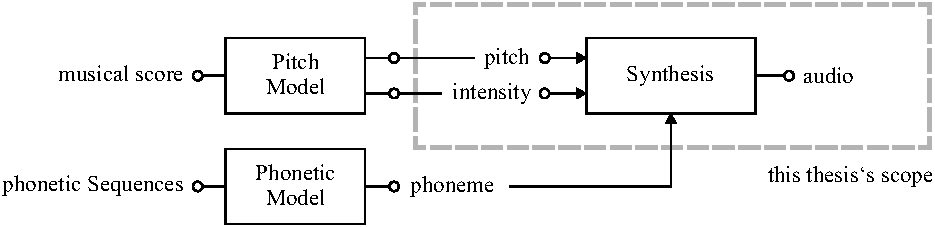
\includegraphics{Graphics/004_thesis_scope.pdf}
    \caption{A text-to-speech singing voice synthesis architecture might consist of a phonetic model, a pitch estimation model and a synthesis model. This thesis scope is limited on the latter.}
    \label{fig:thesis_architecture_scope}
\end{figure}

One possible architecture for a singing voice synthesis model is shown in figure \ref{fig:thesis_architecture_scope}. While the two control parameters pitch and intensity can be controlled directly, they can also be generated from a music score. Phonetic singing voice synthesis methods also include some form of phonetic model, either as a separate component or by conditioning networks using phonemes.\\
In this thesis we want to focus on highly efficient singing voice synthesis, incorporating advances of the past years into classic digital signal processing. To achieve this, this thesis's scope is narrowed down to the synthesis of sung vowels. We therefore do not include a phonetic model or discuss the topic of pitch modelling.
Furthermore, we aim for a multi-singer model, that not only allows voice synthesis using different voice timbre qualities but also morphing between those qualities to create new virtual singers. For analysis, the VocalSet dataset \cite{wilkins_vocalset:_2018} is used to extract pitch and intensity trajectories as well as voice timbre qualities for different virtual singers. This thesis's research questions are as follows:

\begin{itemize}
    \item What methods provide exceptional computational efficiency while still capturing singers voice timbre qualities?
    \item How can we morph efficiently between virtual voices without loosing naturalness?
    \item What validation methods prove suitable for evaluating the naturalness of both synthesized and morphed, synthesized voices.
\end{itemize}

Answering these questions will help us understand important aspects of singing voice synthesis. What might a minimal model for a virtual voice look like that still manages to capture the singers voice qualities? What aspects of a voice are critical for its perception as natural and not synthetic. Application cases for the proposed method can be found in the music software industry. Some scenarios are the implementation of digital choirs or the synthesis of backing or harmonization vocals.\\

With singing voice synthesis being a highly researched topic, the limited scope considered in  this thesis is supposed to help in two ways. Firstly, we aim to differentiate this thesis from existing research. Secondly the limited scope is supposed to reduce the expected workload to a manageable amount, considering the time frame of the thesis of six months and the authors lack of prior knowledge on the topic of singing voice synthesis. \comment{Not sure if this "meta" block is necessary.}


\chapter{Current State of Research}

\section{Voice Production System}

\begin{figure} [H]
    \centering
    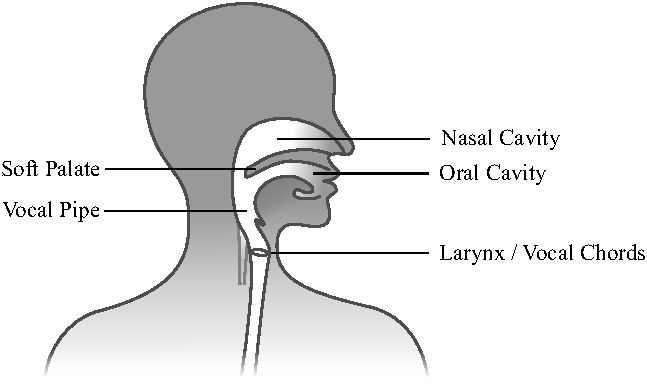
\includegraphics{Graphics/002_VoiceProduction_Physiology.pdf}
    \caption{The human physiology of the organs responsible for the voice production.}
    \label{fig:physiology}
\end{figure}

Early models of the human voice production system were already proposed back in the 1940s \cite{chiba_vowel_1942}. Later on, the source-filter model was widely adopted as a simplified model for the voice production. It was originally proposed in 1960 in \cite{fant_acoustic_1960} but the concept was already explored in experiments with the first vocoder in \cite{dudley_vocoder_1939}, \cite{dudley_remaking_1939}. The source-filter model separates the human voice production in the source and the filter. The source is usually represented by the vocal chords as the organ that initially creates a vibrating air volume, usually referred to as the glottal flow. The filter is represented by vocal tract consisting of the vocal pipe, oral and nasal cavity. The vocal tract filters the glottal flow, creating resonances or formants in the spectrum. \\
There are many ways for a singer to shape the sound. Singers can sing in different registers or phonation modes\cite{sundberg_science_1987} by adjusting the shape of the vocal chords \cite{salomao_what_2009}. The larynx, or voice box, that contains the voice chords, can be moved slightly up and down by singers, shortening or lengthening the vocal tract to alter the filters spectral envelope \cite{sundberg_raised_1976}. By closing the soft palate, singers can decouple the nasal cavity from the remaining vocal tract to again alter the spectral envelope of the filter \cite{elie_characterisation_2009}. Additionally, The singer has control over the filter spectral envelope by shaping the vocal tract, i.e. by moving the tongue or the lips.

\section{Voice Qualities}

In \cite{sundberg_perceptual_1994}, the author classifies voice qualities into timbre, pitch and loudness with timbre qualities being differentiated again in vowel and voice qualities. 
Timbre qualities are mostly controlled by the shape and length vocal tract, and determine the perceived vowel (1st and 2nd formant) and the voice timbre (higher formants). The perceived loudness is not only affected by the overall amplitude but also by the ratio between higher and lower overtone. Temporal variations in pitch, loudness, timbre and phonation are referred to as expression. 

\section{Singing Voice Synthesis}

\begin{figure}[H]
    \centering
    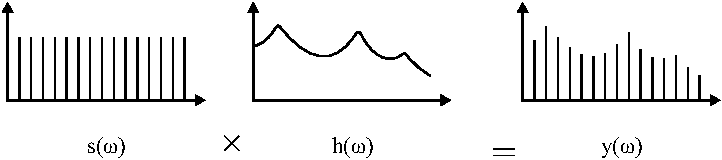
\includegraphics{Graphics/003_SourceFilter_1960.pdf}
    \caption{The source-filter model as proposed in \cite{fant_acoustic_1960}.}
    \label{fig:source_filter}
\end{figure}

Based on early models of the voice production system, some of the first singing voice synthesis methods were source-filter model as described in \cite{fant_acoustic_1960}. The original paper proposes a flat harmonic glottal flow model such as an impulse train as the source $s(\omega)$. The filter $h(\omega)$ could be implemented as an all-pole system that would shaped the vowels formants of the output signal $y(\omega)$ as shown in figure \ref{fig:source_filter}. This model only requires estimation of pitch and the spectral envelope $h(\omega)$. For the purpose of spectral envelope estimation, many methods have been suggested. Linear prediction (LP) was proposed early on \cite{makhoul_linear_1975} with a revised pitch synchronous model (PS LP) proposed in \cite{guerchi_pitch-synchronous_2000}. True Envelope (TE), originally proposed in 1979 \cite{imai_spectral_1979} was rediscovered in 2005 \cite{roebel_efficient_2005}\cite{villavicencio_improving_2006} as one alternative method for spectral envelope estimation. TE iteratively smears the spectrum prior to linear prediction by filtering in the quefreuncy domain to prevent the spectral envelope from overfitting harmonic peaks, an issue commonly seen in LP especially with high pitched signals. More recent methods for spectral envelope estimation include CheapTrick \cite{morise_cheaptrick_2015} or multi frame analysis methods\cite{degottex_simple_2016}.\\

Early on, it was noted that a flat harmonic spectrum is a poor approximation for the glottal flow as the original source-filter model proposed. For that reason, alternative models for the glottal flow, such as the 4-parameter LF model \cite{fant_four-parameter_1985} and the revised 1-parameter LF-$R_d$ model \cite{fant_lf-model_1995} were presented. Source-filter models that see the use of non-flat harmonic signals as the source signal or extend the source-filter model otherwise are usually referred to extended source-filter model. With the introduction of parametric glottal flow models however, the task of separating source and filter is non-trivial. Many methods for source-filter separation were proposed \cite{jinachitra_joint_2005}\cite{degottex_glottal_2010}\cite{perrotin_spectral_2019}. Joint estimation methods provide the means to estimate both source and filter simultaneously. In \cite{loweimi_source-filter_2015}, separation is achieved by analysing trends and fluctuations in the phase domain. Other methods rely on optimization algorithms such as differential evolution \cite{schleusing_joint_2013}.\\

For synthesis of full spoken or sung phrases, concatenative systems \cite{schwarz_concatenative_2006} were proposed. 

\section{Machine Learning in Singign Voice Synthesis}

More recently, machine learning methods for end-to-end singing voice synthesis systems were proposed. These include WaveNet \cite{oord_wavenet:_2016}, an autorregressive neural network that was proposed for the use of text-to-speech or singing voice synthesis. A WaveNet is trained to predict the next sample of an audio sequence and, during generation, uses the predicted sample as it's own input. In \cite{blaauw_neural_2017}, a WaveNet structure was used in conjunction with the WORLD vocoder\cite{morise_world:_2016}. The vocoder extracts spectral envelope coefficients, pitch and an aperiodicity measure from audio and uses the same to recreate the signal. The proposed model uses a modified WaveNet structure to predict the vocoder parameters instead of raw audio. This takes the burden of separating pitch and timbre from the network. As a compromise, any prediction errors in the vocoder analysis or synthesis can't propagate back through the network, resulting in a worse performance than end-to-end approaches \cite{engel_ddsp:_2020}. A similar approach, using Generative Adversarial Networks (GAN) instead of WaveNet for vocoder parameter prediction, is presented in \cite{chandna_wgansing:_2019}. Other approaches include WaveRNN \cite{kalchbrenner_efficient_2018}, based on recurrent neural networks (RNN) and \cite{nakamura_singing_2019}, based on Convolutional Neural Networks.\\

Very recently, differentiable digital signal processing (DDSP) was proposed as a method for combining classical digital signal processing with deep neural networks \cite{engel_ddsp:_2020}. The authors suggested the use of differentiable DSP components such as additive synthesis or FIR filter that could be included in neural networks. The proposed autoencoder architecture uses a decoder to extract pitch, loudness and other latent space control variables from an audio input. The decoder then uses these control variables to predict the coefficients for the DSP components to synthesize the original. Since the dsp components are differentiable, the full architecture can propagate back errors in the synthesized signal and thus can be trained as one network. 


\section{Morphing Singers}

For source-filter models, it was suggested early on that the line spectral frequency (LSF)\cite{itakura_line_1975} representation of all-pole filters shows desirable interpolation characteristics. In \cite{roddy_method_2014} the use of LSF was proposed as a method of morphing between spectral envelopes. 


\chapter{Methods}

\section{Dataset}

This thesis uses the VocalSet dataset \cite{wilkins_vocalset:_2018}. The dataset consists of sung vowel excerpts from 20 singers (9 female, 11 male). For each singer, five vowels are sung in different arrangements (single notes, arpeggios and scales) and different singing techniques (vibrato, straight, breathy,...). 

\section{Singing Voice Synthesis}

\begin{figure}[H]
    \centering
    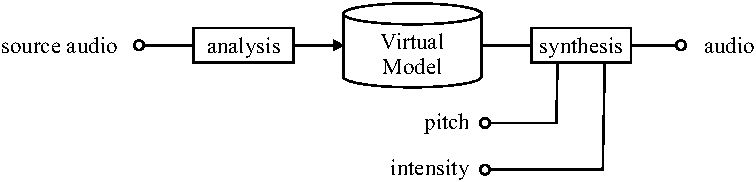
\includegraphics{Graphics/005_method_singer_model.pdf}
    \caption{A singer model is trained from source audio material. The model is used with pitch and control parameters to generate new sung vowels.}
    \label{fig:singer_model}
\end{figure}

In this thesis, we aim to propose a singing voice synthesis method for the synthesis of sung vowels. For this purpose, we train virtual singer model using target source samples from the VocalSet. During synthesis, these models can be used with control parameters pitch and intensity to synthesize new excerpts. Furthermore, singer models can be morphed, either during analysis or synthesis, to blend between voice timbre qualities. An overview is shown in figure \ref{fig:singer_model}.\\

After reviewing the current sate of research, three types of approaches were deemed suitable. These include end-to-end \textbf{audio prediction} approaches like WaveNet \cite{oord_wavenet:_2016}, spectral envelope / \textbf{vocoder prediction} approaches like WGANSing \cite{chandna_wgansing:_2019} and \textbf{extended source-filter} models extracted from source audio \cite{schleusing_joint_2013}. These three  approaches differ in abstraction, required domain knowledge and computational efficiency. Audio prediction methods achieve very good results with low required domain knowledge at the cost of accuracy while extended source filter models require a high level of domain knowledge and perform worse then state at the art methods for the benefit of computational efficiency. A comparison is shown in figure \ref{fig:method_comparison}. In the following sections, all three approaches are briefly introduced. 

\begin{figure}[H]
    \centering
    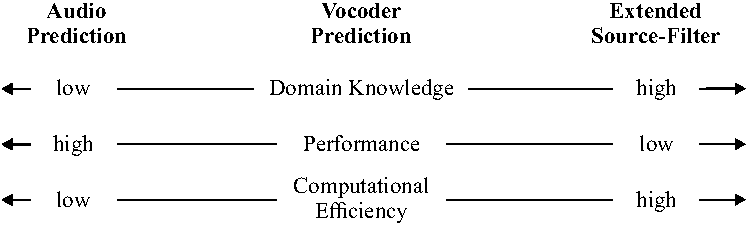
\includegraphics{Graphics/006_method_compairson.pdf}
    \caption{Compared to extended source-filter models, audio predictor approaches trade low required domain knowledge and a better accuracy with a low computational efficiency.}
    \label{fig:method_comparison}
\end{figure}

\subsection*{End-to-End Audio Predictor Methods}

\begin{figure}[H]
    \centering
    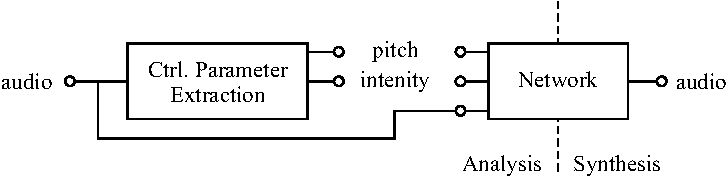
\includegraphics{Graphics/007_method_audio_predictor.pdf}
    \caption{Exemplary architecture of analysis and synthesis of audio predictor  singing voice synthesis methods.}
    \label{fig:method_audio_predictor}
\end{figure}

Audio predictor methods use deep neural networks to predict audio samples based on past predicted audio samples and conditioning signals such as pitch and intensity \cite{oord_wavenet:_2016}. One possible architecture is shown in figure \ref{fig:method_audio_predictor}. During analysis, pitch and intensity trajectories have to be extracted from the source samples. The network is trained to predict new samples in the source audio by observing past samples and the conditioning signals. During synthesis, the network is used to predict new samples based on previously predicted samples (autorregression) and controlled via conditioning signals. A multi singer model can be trained by using multiple singer source samples together with a singer ID one-hot vector as conditioning signal during training. \\
End-to-End audio predictors are usually very complex due to the complexity of the task that the networks are responsible of \cite{engel_ddsp:_2020}.

\subsection*{Vocoder Predictor Methods}

\begin{figure}[H]
    \centering
    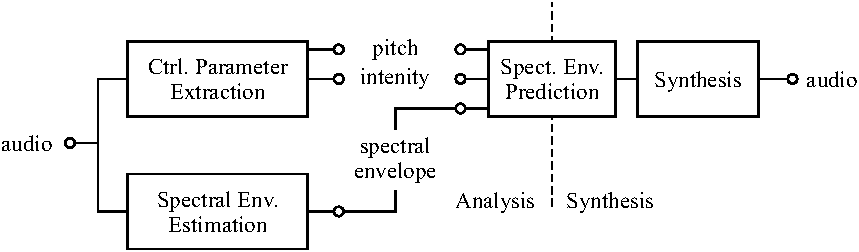
\includegraphics{Graphics/008_method_vocoder_predictor.pdf}
    \caption{Exemplary architecture of analysis and synthesis of vocoder predictor singing voice synthesis methods. }
    \label{fig:method_vocoder}
\end{figure}

Vocoder predictor methods are based on the source-filter model. One possible architecture is shown in figure \ref{fig:method_vocoder}. Instead or predicting raw audio, they predict coefficients for a spectral envelope that can be used together with pitch and additional parameters to synthesize the audio. In  \cite{blaauw_neural_2017-1}, WaveNet was used to the predict the envelope coefficients autorregressively. Various vocoders can be used to extract spectral envelopes and synthesis audio \cite{morise_world:_2016}. One possible advantage over audio predictors is the reduced complexity of predicting spectral envelope parameters \cite{engel_ddsp:_2020}. Having access to spectral envelopes prior to synthesis also allows us to morph between singer models by interpolating between spectral envelopes prior to synthesis, for instance using their LSF representation \cite{roddy_method_2014}. 

\section*{Extended Source-Filter}
    
\begin{figure}[H]
    \centering
    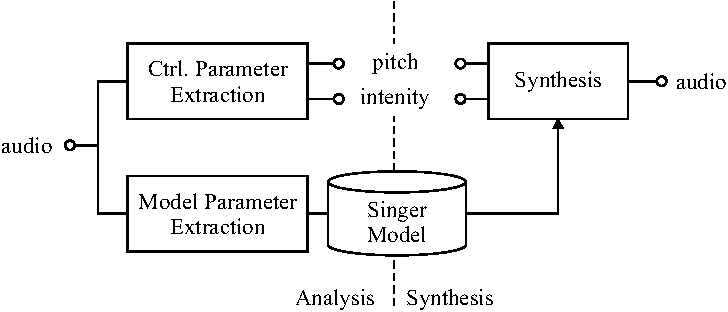
\includegraphics{Graphics/009_method_extended_source_filter.pdf}
    \caption{Exemplary architecture of analysis and synthesis of an extended source filter model for singing voice synthesis methods. }
    \label{fig:method_esf}
\end{figure}

Extended source-filter models require a high level of domain knowledge. The model would not only need to model vocal tract and glottal flow but also would need to model the dependency between control parameters pitch and intensity and the synthesis parameters for vocal tract and spectral envelope. During analysis, all parameters need to be estimated from the source sample. During synthesis, most parts of the model could be implemented using classical signal processing. This dramatically reduces the computational cost compared to the previously presented methods.\\
With vocal tract and glottal flow separated, morphing can be accomplished by interpolating their parameters respectively, again using representations such as LSF to achieve good results.

\subsection*{Differentiable DSP}

DDSP \cite{engel_ddsp:_2020} seems very promising but can't be easily applied to this thesis problem. As mentioned earlier, DDSP combines machine learning with classical DSP but requires the used DSP components to be differentiable. The commonly used model of the vocal tract as an all pole system however is not differentiable. With this limitation, no clean vocal tract separation could be achieved and DDSP could instead only be used to predict coefficients for a sinusoidal plus noise model \cite{serra_musical_1997}.

\subsection*{Summary - Singing Voice Synthesis Methods}

All three presented methods are suitable for implementing singing voice synthesis. However, with the computational complexity of audio prediction and vocoder prediction, an extended source-filter model is the currently preferred method considering the requirements mentioned earlier.\\

\section{Evaluation}

Evaluation of the proposed method is supposed to answer the following questions. Is the proposed method capable of recreating sung vowel excerpts to a satisfactory level? Can the method be used to synthesize sung vowel excerpts perceived as realistic or natural by listeners? Does the proposed model fulfil the strict real time requirements imposed on it? To answer the first two questions, an empirical user test is proposed. Since no hardware is necessary for this test, we suggest conducting an online survey to increase the potential number of participants. 

For measuring the perceived difference between original and synthesized excerpts, a MUSHRA (MUltiple Stimuli with Hidden Reference and Anchor) \cite{itu-r_recommendation_bs.1534_method_2003} test is proposed \cite{morise_cheaptrick_2015}\cite{morise_world:_2016}\cite{blaauw_neural_2017-1}. Alternatively, for small audibly differences, ABC-HR (ABC-Hidden Reference) \cite{itu-r_recommendation_bs.1534_method_2003} can be used instead. The synthesized excerpt is generated using the control parameter trajectories extracted from the original excerpt so that  the synthesized excerpt ideally is perceptually identical to the original excerpt. 

Additionally, some aspects of the method can be evaluated by performing a subjective paired comparison test as proposed in \cite{oord_wavenet:_2016}. In this test, the participants are asked to listen to two samples and state which they prefer with the option to choose "neutral". In all tests, sample $A$ is synthesized directly from model $A$ using the control parameters extracted from the original source audio sample $A$. If the method performs well, we expect a neutral response regarding which sample the participants prefer.

\begin{itemize}
    \item \textbf{Separation of voice timbre qualities and expressive qualities.}\\
    Sample $A$ is compared with an audio sample generated by using the same model $A$ but control parameters extracted from original sample $B$. This test measures how well a model transitions from it's original set of control parameters to a new set of control parameters.  
    \item \textbf{Voice Morphing Capabilities}\\
    The synthesized sample $A$ is compared with the synthesized sample $A \times B$, created by morphing models $A$ and $B$, using the same control parameters as with sample $A$. This test measures how well a morph between models maintains the naturalness of the voice.
\end{itemize}
\chapter{Preparatory Work}

This section describes work conducted in preparation for this master thesis. The biggest portion of which went into researching previous singing voice synthesis methods. Some effort was put into acquiring a better understanding of the human speech production system. A good understanding of the speech production system is important for this thesis mainly for defining a synthesis model that closely mimics the speech production system. Some time was spend studying modern approaches for source filter separation, filter envelope estimation and glottal flow models. The separation of the vocal tract filtering and the vocal folds oscillation (source) is a reoccurring challenge in singing voice synthesis. Finally, some time was devoted to researching machine learning approaches to singing voice synthesis.

In preparation for this thesis, some of the methods proposed in previous papers, including filter envelope estimators (LPC, TE) and glottal flow models (LF, LF-Rd) have been implemented in Matalb in order to get familiar with their performance, strengths and weaknesses. A framework for extract pitch, overtone frequencies and phases of sung vowel excerpts have been implemented using the programming environment Matlab. It was used to explore the VocalSet dataset\cite{wilkins_vocalset:_2018} and to analyse the included singing voice experts regarding spectral content and temporal fluctuation of pitch and overtone amplitude and phase. 


\chapter{Work and Timetable}

This section outlines the timetable for the thesis. The preparatory work prior to the thesis application included researching state of the art singing voice synthesis methods and defining the research questions. The main phase of the thesis consists of implementation, evaluation and thesis writing. The singing voice synthesis method is realized in an iterative manner with the implementation going hand in hand with additional research and intermediate evaluation phases. The final evaluation phase consists of an empirical test and is intended to validate the synthesis method on a perceptual level. Writing is supposed to last one month. Two months are reserved as optional time in case any of the other phases take longer then expected. A time schedule is provided in table \ref{table:time_schedule};

\begin{table}[H]
  \centering
    \renewcommand{\arraystretch}{1.5}
  \begin{tabular}{c | c ? c | c |c | c ? c | c}
  \hline
    January & February & March & April & May & June & July & August \\\hline 
    \multicolumn{2}{c?}{Preparatory} & \multicolumn{4}{c?}{Thesis} & \multicolumn{2}{c}{Buffer}\\\hline
    Research & Proposal & \multicolumn{2}{c|}{Implementation} & \multicolumn{1}{c|}{Evaluation} & \multicolumn{1}{c?}{Writing} & \multicolumn{2}{c}{}\\\hline 
  \end{tabular}
  \caption{The proposed work time plan for the master thesis.}
  \label{table:time_schedule}
\end{table}

\section{Agenda}

This section roughly outlines the remaining tasks that comprise this thesis.

\subsection*{Preparatory Work}
\begin{itemize}
    \item Compile and summarize prior research in the field of singing voice synthesis.
    \item Write the exposé for the thesis application.
\end{itemize}

\subsection*{Implementation}
\begin{itemize}
    \item Define a method following the requirements laid out in this document.
    \item Iterative prototyping of the proposed method, conducting additional research and evaluation phases when necessary. 
    \item Source code refactoring and documentation.
\end{itemize}


\subsection*{Evaluation}
\begin{itemize}
    \item Compile material (synthesized and original audio excerpts) for the empirical test
    \item Design an empirical test / online survey
    \item Implement the online survey using tools such as LimeSurvey
    \item Run and maintain the survey
    \item Collect and analyse test results 
\end{itemize}

\subsection*{Writing}
\begin{itemize}
    \item Write the master thesis 
    \item Write German summary of the thesis
    \item Iterative proofreading and improving of content and writing
    \item Final proofreading and spellchecking
\end{itemize}



%--------------------------------------------------------------
% Body Matter abschließen
% Seitenzahl übertragen auf Backmatter
\newcounter{Seitenzahl}
\addtocounter{Seitenzahl}{\value{page}}
\clearpage

%--------------------------------------------------------------
% Back Matter - Abbildungs- und Tabellenverzeichnis, Listings, Index, Glossare, etc.
% Römische Zahlen für Back Matter - Seitenzahl an Front Matter anschließen
\pagenumbering{arabic}
\addtocounter{Seitenzahl}{1}
\setcounter{page}{\value{Seitenzahl}}

% Wenn gewünscht, Verzeichnis der Listings auskommentieren
%\lstlistoflistings

% Diesen Schalter einbinden, wenn Symbole, Abkürzungen, etc. ohne Referenz im Dokument in den 
% Verzeichnissen eingebunden werden sollen (meistens der Fall)
%\glsaddall

% Wenn gewünscht, Glossar auskommentieren (wird nur erstellt, wenn Einträge verfügbar)
%\printglossary

% Wenn gewünscht, Abkürzungen auskommentieren (wird nur erstellt, wenn Einträge verfügbar)
%\printglossary[type=\acronymtype,style=list]

% Wenn gewünscht, Symbole auskommentieren (wird nur erstellt, wenn Einträge verfügbar)
%\printglossary[type=symbols, style=symb3spaltig, nonumberlist]

% Wenn gewünscht, Index auskommentieren
%\printindex

% Wenn gewünscht, Literaturverzeichnis auskommentieren

%Alle Quellen, ob genutzt oder nicht, werden ausgegeben
%\nocite{*}


%Das kein Seitenumbruch stattfindet
\interlinepenalty 10000

%\bibliography{Content/Bibliographie}

% Changed by Max W.
\renewcommand{\bibname}{Literature}
\bibliography{Content/Bibliographie/zotero_references.bib}

% Anhang
%\appendix
%\input{Content/Appendix.tex}


% Back Matter abschließen
\clearpage

%--------------------------------------------------------------
% Anhang
%\input{Content/Appendix.tex}

\end{document}
